% !TeX spellcheck = fr_FR
\thispagestyle{noheader}
\chapter*{Résumé} % No (numbered) toc entry with *

\tikz[remember picture,overlay] \node[shift={(4.165cm,-1.955cm)}]
	at (current page.north west)
	{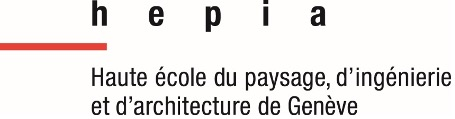
\includegraphics[height=1.29cm]{template/images/title/hepia_logo}};
	\tikz[remember picture,overlay] \node[shift={(-4.238cm,-1.97cm)}]
	at (current page.north east)
	{
\includegraphics[height=1.29cm]{template/images/title/hes-so_geneve_logo}};

\addcontentsline{toc}{chapter}{Résumé} % Adding toc entry
\thispagestyle{noheader}

\begin{spacing}{0.92}
\vspace{-0.5cm}

	%% CONTENT STARTS HERE
Ce projet vise à synchroniser les arrêts de transport public présents dans OpenStreetMap (OSM) avec ceux du système officiel suisse ATLAS, afin d’améliorer la précision et la fiabilité des données. Nous analysons d’abord la structure, la couverture et les balises des deux sources (ATLAS/OSM) en Suisse, en mobilisant les jeux GTFS et HRDF pour caractériser les lignes et leurs directions.

Nous mettons ensuite en place un pipeline d’appariement séquentiel combinant plusieurs méthodes (exacte, par nom, par distance, par lignes GTFS/HRDF), suivi d’une consolidation et de la gestion des doublons. Parmi \textbf{55\,571} arrêts ATLAS, nous établissons \textbf{48\,419} correspondances, soit \textbf{84,3\%} d’arrêts ATLAS distincts appariés. Répartition par méthode : \textbf{21\,237} exactes, \textbf{18\,618} par distance, \textbf{7\,021} par lignes, \textbf{537} par nom.

Un système de \textbf{détection et de priorisation des problèmes} met en évidence \textbf{16\,408} anomalies de priorité \textbf{P1} (distance : \textbf{1\,171} ; non-appariements : \textbf{8\,192} ; attributs : \textbf{7\,045}), guidant la revue ciblée.

Nous développons une application web permettant de visualiser les deux ensembles et leurs correspondances, de produire des rapports, de corriger les problèmes détectés et d’effectuer des correspondances manuelles avec \textbf{persistance} des décisions.

Enfin, l'application intègre un volet de sécurité aligné sur les bonnes pratiques (mots de passe Argon2, 2FA TOTP, CSRF, limitation de débit) et une conteneurisation Docker assurant un déploiement reproductible.  L'ensemble constitue une base pour améliorer durablement la qualité des données et accélérer la synchronisation OSM–ATLAS.

\vspace{0.2cm}
\begin{figure}[h]
\centering
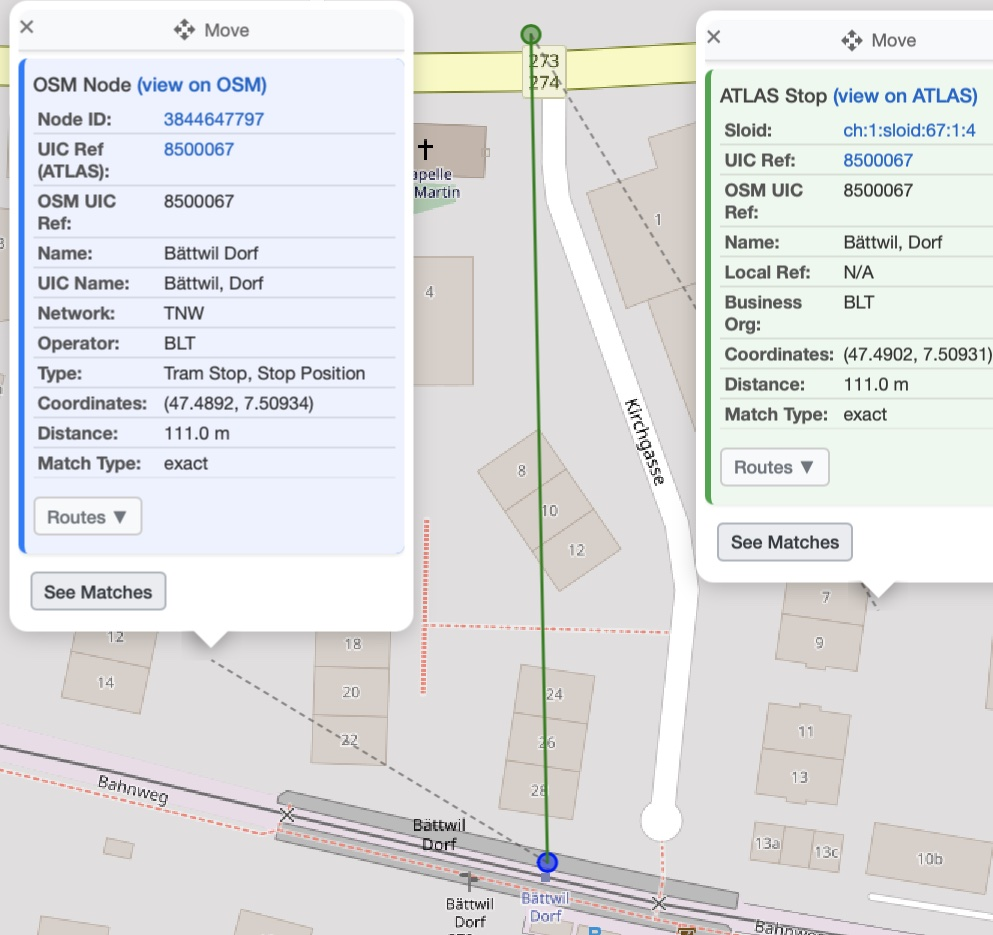
\includegraphics[width=0.45\textwidth]{figures/abstract.jpg}
\caption*{Exemple de problème de priorité 1~: Bättwil, Dorf}
\end{figure}
\vspace{0.1cm}

\vfill
\begin{center}

\vfill
%% CONTENT ENDS HERE

{
%%%%%%%%%%%%%%%%%%%%%%%%%%%%%%%%%%%%%%%%%%%%%%%%%%%%%%%%%%%%%%%%%%%%%%%%%%%%%%%%
%%%%%%%%%%%%%%%%%%%%%%%%%% DO NOT MODIFY THE TABLE BELOW %%%%%%%%%%%%%%%%%%%%%%%
%%%%%%%%%%%%%%%%%%%%%%%%%%%%%%%%%%%%%%%%%%%%%%%%%%%%%%%%%%%%%%%%%%%%%%%%%%%%%%%%
	\begin{tabular*}{16cm}{p{7.59cm} p{7.58cm}}
		\small Candidat-e:					&	\small Professeur-e(s) responsable(s):\\*[4pt]
		\small\textbf{\textsc{\Author}}		&	\small\textbf{\textsc{Orestis MALASPINAS}}\\*[4pt]
		\footnotesize  Filière d'études: ISC	&	\footnotesize  \textbf{En collaboration avec:} SKI+\\*[4pt]
		\footnotesize  {} & \footnotesize  Travail de bachelor soumis à une convention de stage en entreprise: non \\*[4pt]
		\footnotesize  {} & \footnotesize  Travail soumis à un contrat de confidentialité: non\\*[4pt]
	\end{tabular*}\\*[1.cm]
}
	
\end{center}
\end{spacing}
